\section{Cálculo de parámetros $\frac{W}{L}$ \label{sec:s1}}

\begin{center}
	\begin{minipage}{12cm}
		\begin{tcolorbox}[title=Actividad 1]
			Emplear la siguiente metodología, propuesta por \cite{Allen_2012} para diseñar el amplificador simple de una etapa (Ver \autoref{fig:calculos_allen}).
		\end{tcolorbox}	
	\end{minipage}
\end{center}

\begin{figure}[H]
	\centering
	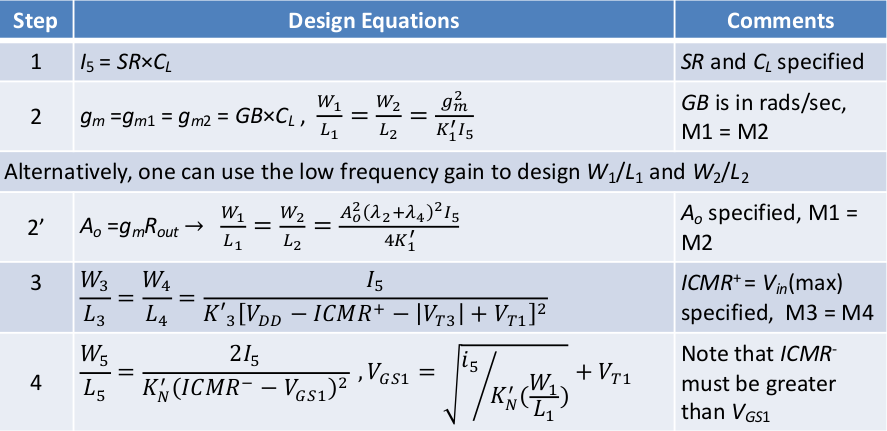
\includegraphics[scale=0.5]{Calculos_Allen.png}
	\caption{Procedimiento de diseño. \label{fig:calculos_allen}}
\end{figure}

\begin{equation*}
	\begin{array}{l l}
		\textbf{Parámetros conocidos} \\
		V_{DD} =  1.8  V \\
		L_{min} =  150.0  nm \\
		0.7 V \leq ICMR \leq 1.6 V \\
		K'_{N} =  151.37604  \frac{\mu A}{V^{2}} \\
		K'_{P} =  57.013889  \frac{\mu A}{V^{2}} \\
		V_{TN} =  0.769432  V \\
		V_{TP} =  0.624345  V \\
		\lambda_{N} =  0.088964  V^{-1} \\
		\lambda_{P} =  0.068964  V^{-1} \\
		C_{L} =  12.0  pF \\
		\\
		\textbf{Características deseadas} \\
		A_{V} =  100  \frac{V}{V} \\
		P_{diss} \leq  1  mW \\
		GB =  10.0  MHz \\
		SR \geq  5  \frac{V}{\mu s} \\
		\\
		\textbf{Paso 1} \\
		I_{5} = SR \times C_{L} = 5\times1.2e-11 \\
		I_{5} =  60.0 \mu A \\
		\\
		\textbf{Paso 2} \\
		g_{m} = 2\pi{} \times GB \times C_{L} = 2 \pi{} \times10000000.0\times 1.2e-11  \\
		g_{m} =  753.982237  \mu S \\
		\frac{W_1}{L_1} = \frac{gm^2}{K'_{N}\times I_5} = \frac{0.000754^2}{0.000151\times6e-05}\\
		\frac{W_1}{L_1} =  62.591281  \\
		W_{1} = \frac{W_1}{L_1} \times L_{min} =  62.591281 \times 1.5e-07  \\
		W_{1} = W_{2} =  9.388692  \mu m \\
		\\
		\textbf{Paso 3} \\
		\frac{W_3}{L_3} = \frac{I_5}{K'_{P}\times \left[(V_{DD}-ICMR^{+}-|V_{TP}|+V_{TN}\right]^{2}} = \frac{ 6e-05 }{ 5.7e-05 \times \left[ 1.8 - 1.6 - 0.624345 + 0.769432 \right]^{2}} \\
		\frac{W_3}{L_3} =  8.837174  \\
		W_{3} = \frac{W_3}{L_3} \times L_{min} =  8.837174 \times 1.5e-07  \\
		W_{3} = W_{4} =  1.325576  \mu m \\
	\end{array}
\end{equation*}

\begin{equation*}
	\begin{array}{l l}
		\textbf{Paso 4} \\
		V_{GS1} = \sqrt{\frac{I_{5}}{K'_{N}\times\frac{W_{1}}{L_{1}}}}+V_{TN} = \sqrt{\frac{ 6e-05 }{ 0.000151 \times 62.591281 }}+ 0.769432  \\
		V_{GS1} =  0.849009  V \\
		\frac{W_{5}}{L_{5}} = \frac{2\times I_{5}}{K'_{N}\times (ICMR^{-}-V_{{GS1}})^{2}} = \frac{2\times 6e-05 }{ 0.000151 \times ( 0.7 - 0.849009 )^{2}} \\
		\frac{W_5}{L_5} =  35.702313  \\
		W_{5} = \frac{W_5}{L_5} \times L_{min} =  35.702313 \times 1.5e-07  \\
		W_{5} = W_{6} =  5.355347  \mu m \\
		\\
		\textbf{Paso 5} \\
		A_{0} = \frac{2g_{m}}{(\lambda_{N}+\lambda_{P})\times I_{5}} = \frac{2\times 0.000754 }{( 0.088964 + 0.068964 )\times 6e-05 } \\
		A_{0} =  159.141041  =  44.035644  db \\
		\\
		\textbf{Parámetros calculados} \\
		W_{1} = W_{2} =  9.388692  \mu m \\
		W_{3} = W_{4} =  1.325576  \mu m \\
		W_{5} = W_{6} =  5.355347  \mu m \\
		L_{1} = L_{2} = L_{3} = L_{4} = L_{5} = L_{6} = 0.15  \mu m \\
	\end{array}
\end{equation*}